%% Lab Report for EEET2493_labreport_template.tex
%% V1.0
%% 2019/01/16
%% This is the template for a Lab report following an IEEE paper. Modified by Francisco Tovar after Michael Sheel original document.


%% This is a skeleton file demonstrating the use of IEEEtran.cls
%% (requires IEEEtran.cls version 1.8b or later) with an IEEE
%% journal paper.
%%
%% Support sites:
%% http://www.michaelshell.org/tex/ieeetran/
%% http://www.ctan.org/pkg/ieeetran
%% and
%% http://www.ieee.org/

%%*************************************************************************
%% Legal Notice:
%% This code is offered as-is without any warranty either expressed or
%% implied; without even the implied warranty of MERCHANTABILITY or
%% FITNESS FOR A PARTICULAR PURPOSE! 
%% User assumes all risk.
%% In no event shall the IEEE or any contributor to this code be liable for
%% any damages or losses, including, but not limited to, incidental,
%% consequential, or any other damages, resulting from the use or misuse
%% of any information contained here.
%%
%% All comments are the opinions of their respective authors and are not
%% necessarily endorsed by the IEEE.
%%
%% This work is distributed under the LaTeX Project Public License (LPPL)
%% ( http://www.latex-project.org/ ) version 1.3, and may be freely used,
%% distributed and modified. A copy of the LPPL, version 1.3, is included
%% in the base LaTeX documentation of all distributions of LaTeX released
%% 2003/12/01 or later.
%% Retain all contribution notices and credits.
%% ** Modified files should be clearly indicated as such, including  **
%% ** renaming them and changing author support contact information. **
%%*************************************************************************

\documentclass[a4paper, technote, compsoc]{IEEEtran}
% \documentclass{article}

% *** CITATION PACKAGES ***
\usepackage[backend=biber,style=ieee]{biblatex} 
\bibliography{biblio.bib}
   %your file created using JabRef

% *** MATH PACKAGES ***
\usepackage{amsmath}

% *** PDF, URL AND HYPERLINK PACKAGES ***
\usepackage{url}
% correct bad hyphenation here
\usepackage{graphicx}  %needed to include png, eps figures
\usepackage{float}  % used to fix location of images i.e.\begin{figure}[H]

\usepackage[utf8]{inputenc} % allow utf-8 input
\usepackage[T1]{fontenc}    % use 8-bit T1 fonts
\usepackage{xcolor}
\usepackage{booktabs}
\usepackage{mwe}

\begin{document}

% paper title
\title{Reduced Order Models \\ With Moving Domains \\ \normalsize{Research Project}}

% author names 
\author{Enrique Millán Valbuena \\ \normalsize{463 426 8}}% <-this % stops a space
        
% The report headers
\markboth{M. Sc. Aerospace Engineering, TU Delft}%do not delete next lines
{Shell \MakeLowercase{\textit{et al.}}: Bare Demo of IEEEtran.cls for IEEE Journals}

% make the title area
\maketitle

% As a general rule, do not put math, special symbols or citations
% in the abstract or keywords.
\begin{abstract}
   The research objective is to build a reduced order model for a parametrized heat diffusion problem with a moving boundary. 
   Physical and geometrical parameters are considered.

   A concise description of the reducing procedure is provided, together with a posteriori error estimators to certify their use and a numerical example to showcase computational costs and implementation details. 
\end{abstract}

\begin{IEEEkeywords}
Reduced basis methods, moving domain, heat equation, FEM, DEIM, MDEIM, POD, Galerkin-projection
\end{IEEEkeywords}

\section{Introduction}
The MSc Thesis focuses in the fast solution of parametrized linear parabolic PDEs with moving boundaries.
For the sake of clarity, we shall now state the problem without too much mathematical formalism, which we shall keep for later.

Parametrized PDEs can be numerically solved with the Finite Element Method (FEM), which lead to an algebraic system of equations whose solution can be computationally expensive to obtain, specially for complex geometries or detailed models.
When this is the case, many-query procedures and access to field values or calculated outputs for different parameter values $\mu$ can become cumbersome, or even infeasible due to computational costs, both in time and memory.
One often refers to this FEM model as the \textit{Full Order Model}~(FOM),
\begin{equation*}
   \frac{du_h}{dt} + A_h\left(t;\mu\right) u_h = f_h\left(t;\mu\right).
\end{equation*}

To circumvent these issues, one can build a \textit{Reduced Order Model}~(ROM), whose solution is fast in time and light in storage.
This ROM is based in ad-hoc empirical basis functions, whose support typically spans the whole domain. 

\subsection{Brief Outline Of The Reduction Process}
The construction of the ROM has mainly two phases:
\begin{itemize}
   \item Offline phase: construction of the ROM.
   \item Online phase: usage of the ROM.
\end{itemize}

During the offline phase, the costly algebraic problem is solved for a subset of the parameter space.
Snapshots of the matrices, vectors and solutions are stored and processed via algebraic reduction algorithms, in order to obtain a reduced basis for each of them.
An example of reduction algorithms would be the Discrete Empirical Interpolation Method (DEIM) and its matrix version (M-DEIM).

The offline phase scales with the dimension of the Full Order Model, $N_h$, which is governed by the number of nodes in the mesh and the polynomial degree for the FEM basis.
Once the offline phase is over, a representative basis for each operator of the algebraic problem has been produced, of representative size~$N \ll N_h$\footnote{The reduction of each operator might have required a different number of basis elements, but they should be all of the same order of magnitude or smaller for the reduction procedure to be a success.}.

These bases are later used during the online phase, where for new parameters a small algebraic system is built and solved,
\begin{equation*}
   \frac{du_N}{dt} + A_N\left(t;\mu\right) u_N = f_N\left(t;\mu\right).
\end{equation*}
In this stage, it is paramount to allow for an assembly of the operators\footnote{
   We shall abuse notation and refer to the operators for both the matrices and the functionals, unless explicit distinction is required.
} 
independent of the original problem size $N_h$.
When this is the case, we state to have an \textit{
   ideal offline-online decoupling}.

An essential ingredient to achieve such decoupling is what we call an \textit{
   affine decomposition} 
of the problem operators.
Simply put, it is to say that we can achieve linear separation in the parameters and the operator algebraic representation, 
\begin{equation*}
   A_h\left(t;\mu\right) = \sum_{q=1}^{Q} \Theta_{q}(t;\mu) A_{h,q},
\end{equation*}
where~$A_{h,q}$ are constant matrices and~$\Theta_{q}(t;\mu)$ are scalar values. 

The easiest example one could come up with of an affine decomposition is the one present in the heat diffusion problem with two different but constant diffusion parameters $k_q$ across the domain.
Then, the affine decomposition would look like
\begin{equation*}
   A_h\left(t;k_1, k_2\right) = k_{1} A_{h,1} + k_{2} A_{h,2},
\end{equation*}
where each matrix $A_{h,q}$ would represent the diffusion operator with support over the subdomain associated with each parameter. 
For this simple example, the affine decomposition is present naturally, but it will not always be the case, specially when non-linearities are present. 

However, nowadays it is absolutely possible to obtain an automatic ad-hoc affine decomposition of any operator thanks to grounded algorithms and procedures, like DEIM and MDEIM.
This key fact will allows us to achieve a perfect split between the offline and the online phase, as it will allow us to assemble our ROM operators without having to assemble at any point the complete FOM operator. 

Finally, once the problem the reduced has been solved, the solution can be projected back to the original mesh. 

In this way, access to field values or calculated outputs can be obtained lightly, provided the overall procedure is \textit{certified}: to prove in the online phase without solving the FOM that the solution is sufficiently close to what would have been if the actual FOM had been assembled and solved.

% Ideally, 
%% Research objectives
% Useful: benefit of your research to the problem. 
% Realistic: contribute to the solution of the problem.
% Feasible: time scheduled and capabilities and resources.
% Clear: be precise in the contribution to the problem.
% Informative: rough idea of knowledge generated towards a solution.

% The research objective is (a) by (b).
% (a) The contribution of the research project to the solution of the problem.
% (b) description of the way the contribution will be provided. 

\begin{figure}[h]
   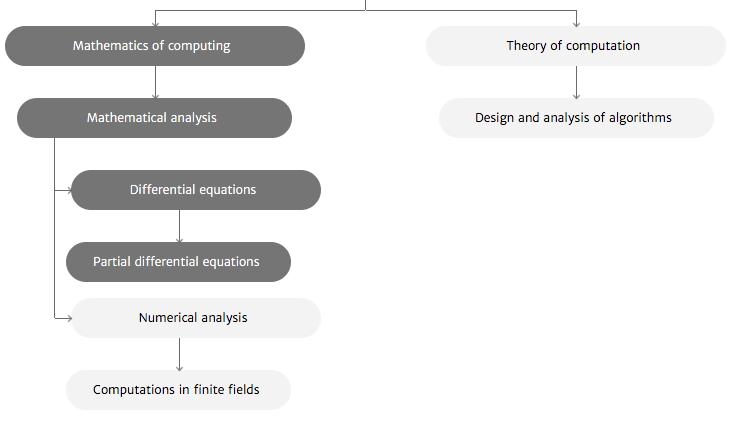
\includegraphics[width=\columnwidth]{figures/index.png}
   \caption{Conceptual location of the research project.}
\end{figure}

\subsection{A Note On The Word \textit{Linear}}
A non-linearity is essentially a characteristic that prevents a linear separation.

Despite the apparent linear character in algebra of the target equation, it is actually non-linear.
The introduction of the time variable~$t$~in the shape of the domain changes the operators at each time step during the integration procedure. 
Additionally, since the domain geometry will depend in some parameter values too, one cannot explicitly split the domain.  

Another type of non-linearity would be a term whose value depended on the field function $u$. 
These kind of non-linearities are common in mathematical modelling, but 




\section{Objectives and goals}
The research objective is to build a reduced order model for a parametrized heat diffusion problem with a moving boundary, 
by providing a concise description of the reducing procedure, 
a posteriori error estimators to certify their use and 
a use case to showcase computational costs and implementation details. 

Both the main equation of the PDE and the geometrical definition of the moving boundary are parametrized. 

\subsection{Scope}
A non-linearity is essentially a characteristic of a problem that prevents a linear separation.
Despite the apparent linear character of the naive heat equation, it is actually non-linear, since the introduction of the time variable $t$ in the domain changes the operators at each step. 

Another type of non-linearity would be a term whose value depended on the field function $u$. 
These kind of non-linearities are common in mathematical modelling, but 

We shall limit our research to this kind of problem, without the introduction of further non-lineariti

The project is mainly practice-oriented, in that we shall design, build and evaluate the procedure to construct the ROM.
Many reduction tools and strategies are available nowadays, each of them with their benefits and drawbacks. 



we intend to have theoretical content too.

By introducing the construction of a posteriori error estimators\footnote{Which rely on the usual stability factors and arguments present in Finite Element techniques.}, one can certify the results of the reduced basis for unseen in the training phase parameters.

%% Theory-oriented
% Theory development
% Theory testing

%% Practice-oriented: intervention cycle
% Problem Analysis
% Diagnosis
% Design
% Change
% Evaluation


%% Research Strategy
% Suitability
% Duration
% Feasibility



\newpage
\section{Conclusions}
\label{sec:conclusions}

\printbibliography

% http://danceswithcode.net/engineeringnotes/rotations_in_3d/rotations_in_3d_part1.html

\end{document}


